\documentclass[a4paper]{article}

\usepackage[english]{babel}
\usepackage[utf8]{inputenc}
\usepackage{amsmath}
\usepackage{graphicx}
\usepackage[colorinlistoftodos]{todonotes}
\usepackage{authblk}
\usepackage{fancyhdr}
\usepackage[headheight=25pt]{geometry}
\usepackage{lastpage}
\usepackage[title]{appendix}
\usepackage{float}

\pagestyle{fancy}

\fancyhead[L]{\footnotesize STAT 413: INTRODUCTION TO STATISTICAL MACHINE 
LEARNING \\ GENEVERA I. ALLEN}
\fancyhead[R]{\footnotesize 2017-2018, FALL SEMESTER \\ RICE UNIVERSITY}
\fancyfoot[L]{\footnotesize HOMEWORK 0: KNN, MLR, MVS \\ MICHAEL RODGERS}
\fancyfoot[R]{\footnotesize Page \thepage\ of \pageref{LastPage}}
\fancyfoot[C]{}

\graphicspath{{figs/}}

\title{hw0}

\author[1]{Michael Rodgers}
\affil[1]{Rice University}

\date{\today}

\begin{document}
\maketitle

\begin{abstract}
This will be my homework template. With the template I can upload pictures 
of graphs and screen shots of tables (if needed). My netid is mjr10.
\end{abstract}

\section{Problem 1}

According to figure \ref{fig:mspe} in the Appendix, we see this. I can now 
reference a figure in the appendix. Now I need to learn to type math 
equations in latex properly. 

\newpage

\section{Problem 2}

This is the layout for a new page. The header and footer are worthwhile.

\newpage

\begin{appendices}
\section{Figures}

\begin{figure}[H]
\begin{center}
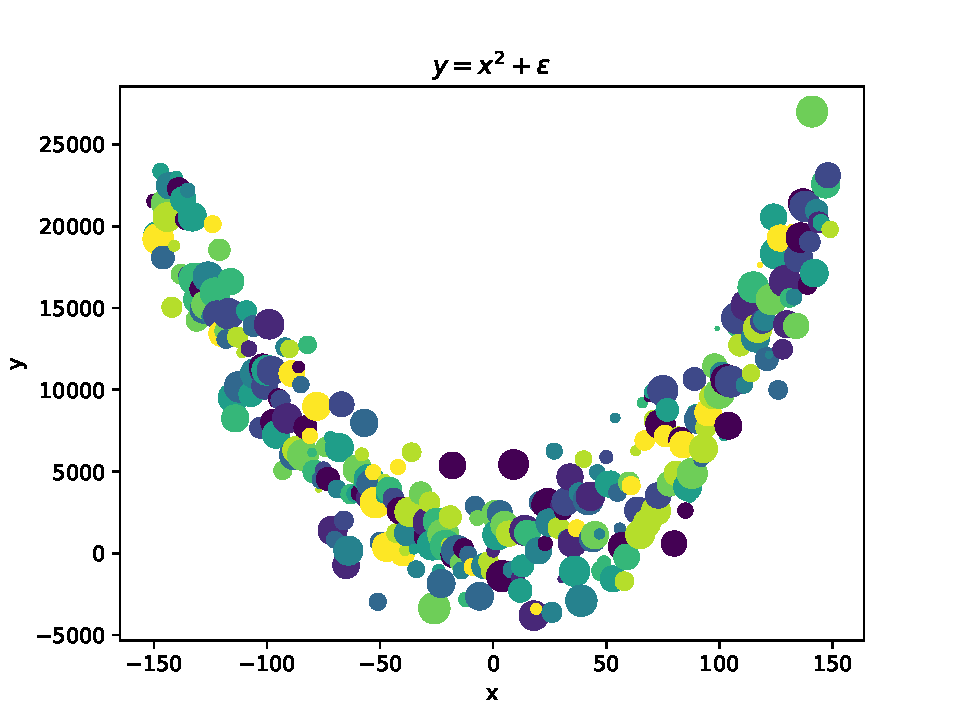
\includegraphics[width = 5in]{mike.pdf}
\caption{mspe}
\label{fig:mspe}
\end{center}
\end{figure}
 % add figs at the end of the file

\end{appendices}

\end{document}